\chapter{Implementação}

Para validar o conceito apresentado nos capítulos anteriores, a arquitetura do \textit{framework} foi implementada em uma forma minimalista. Alguns detalhes do \textit{framework} foram simplificadospara esta implementação, umas vez que se trata de uma prova de conceito.

Neste capítulo serão tratados detalhes de implementação do framework de simulação, particularidades de implementação e decisões de \textit{design} de software, assim como alguns exemplos de aplicação e utilização do framework.

Para esta implementação foi utilizada a linguagem \textit{Python}. Toda a comunicação entre máquinas distintas foi feita utilizando \textit{sockets} sobre o protocolo \textit{TCP}. As tarefas assíncronas da implementação foram contruídas sobre a implementação de nativa \textit{threads} provida pela própria linguagem.

\section{A linguagem \emph{Python}}

Python é uma linguagem de programação poderosa e de fácil aprendizado. Possui estruturas de dados de alto nível eficientes, bem como adota uma abordagem simples e efetiva para a programação orientada a objetos. Sua sintaxe elegante e tipagem dinâmica, além de sua natureza interpretada, tornam Python ideal para scripting e para o desenvolvimento rápido de aplicações em diversas áreas e na maioria das plataformas.

O interpretador Python e sua extensa biblioteca padrão estão disponíveis na forma de código fonte ou binário para a maioria das plataformas \cite{PYTHONSITE}, e podem ser distribuídos livremente. Também estão disponíveis distribuições e referências para diversos módulos, programas, ferramentas e documentação adicional, contribuídos por terceiros.

O interpretador Python é facilmente extensível incorporando novas funções e tipos de dados implementados em C ou C++ (ou qualquer outra linguagem acessível a partir de C). Python também se adequa como linguagem de extensão para customizar aplicações.

A linguagem vem sendo amplamnete empregada em desenvolvimento na área de computação científica devido ao seu desempenho satisfatório e sua facilidade de uso. Mais detalhes sobre a linguagem são tratados no apêndice~\ref{appendix_python}.

\section{As camadas externas}

A arquitetura apresentadas nos capítulos anteriores deste documento é representada pelo diagrama \textit{UML} da figura~\ref{fig:arquitetura_uml_geral} (Uma versão expandida, portanto mais completa, deste diagrama encontra-se no anexo~\ref{appendix_uml_completo}). Vale ressaltar que esta representação é completamente independente da linguagem escolhida para sua implementação, porém atrelada ao paradigma de programação orientado à objetos, eleito para construir o \textit{framework} de simulação.

A arquitetura da árvore de diretórios de como foi implementado o \textit{framework} é ilustrada no apêndice~\ref{appendix_tree}. A partir dela pode-se ilustrar a modularização dos componentes do projeto e a divisão dos módulos do \textit{framework}. Os módulos são descritos a seguir:

\begin{itemize}
\item \textbf{doc:} Contém toda a documentação do projeto, inclusive esta monografia.
\item \textbf{examples:} Contém exemplos de aplicação do \emph{framework}.
\item \textbf{setup.py:} \emph{Script} de instalação do \textit{framework}.
\item \textbf{t100:} Código fonte do \textit{framework}.
\end{itemize}

Nas seções seguintes são apresentados detalhes internos da estrutura do código implementado, do subdiretório \textit{t100}. 

\subsection{Módulos internos do \emph{framework}}

\begin{figure}
  \centerline{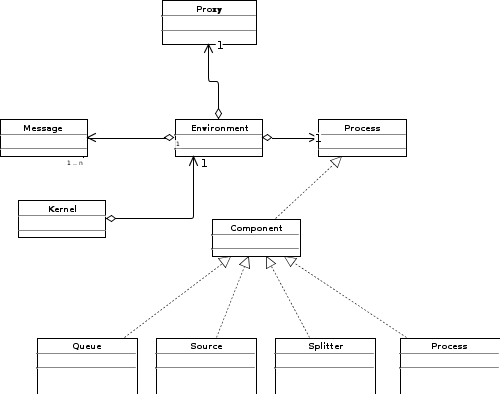
\includegraphics{arquitetura_uml_geral.png}}
  \caption{Diagrama simplificado de classes do \textit{framework}.}
\label{fig:arquitetura_uml_geral}
\end{figure}

O código fonte do \textit{framework} pode ser dividido inicialmente em quatro grandes módulos:

\begin{itemize}
\item \textbf{components:} Possui toda a descrição dos componentes utilizáveis na simulação.
\item \textbf{core:} O módulo \textit{core} possui todos os principais algorítmos internos ao \textit{framework}. São os algorítmos não-modularizáveis do projeto.
\item \textbf{simtool:} O módulo \textit{simtool} possui as implementações de algorítmos modularizáveis do projeto. Neste caso entram algorítmos de sincronismo, de troca de mensagens, etc.
\item \textbf{test:} São os \textit{scripts} de testes do sistemas, necessários para validar a integridade do projeto após eventuais mudanças no código.
\end{itemize}

O módulo \textit{core} possui as especificações mínimas que descrevem componentes e o \textit{kernel} do simulador. São encapsulados também neste nível dados algumas classes de manipulação de erros e algoritmos básicos de execução.

O módulo \textit{components} possui a implementação base necessária para se descrever um componente para a simulação, além de componentes genéricos. Mais detalhes sobre este módulo são tratados na seção~\ref{implement_components}.

\section{Implementando a comunicação}

A linguagem de programação \textit{Python} oferece uma ampla e funcional biblioteca padrão, que provê, de forma nativa na linguagem, métodos para implementação de \textit{threads, sockets}, persistência de dados e estruturas de dados.

Conforme ilustrado na figura~\ref{fig:uml_proxy_basico}, o proxy mínimo de comunicação deve oferecer os seguintes métodos: \textit{send, receive, listen}.

Para a implementação da camada de comunicação do \textit{framework} de simulação, foi adotada uma estratégia simplista, utilizando-se das bibliotecas de comunicação disponibilizadas pela linguagem adotada.

Toda a comunicação se faz por meio de troca de mensagens utilizando \textit{sockets} sobre o protocolo \textit{TCP/IP}.

\subsection{O objeto \emph{Message}}

Toda a comunicação entre instâncias de \textit{proxy} é realizada enviando e recebendo objetos do tipo \textit{Message}. Um objeto do tipo \textit{Message} é um objeto obrigatoriamente serializável (ou seja, ele pode ser convertido de objeto para um \textit{stream} de bytes a qualquer instante do seu ciclo de vida. Este \textit{stream} de \textit{bytes} deve ser usado para reconstruir o objeto \textit{Message}).

O objeto possuim os campos \textit{content}, que é o conteúdo da mensagem propriamente dito, além dos campos de endereço lógico do remetente e do destinatário. Cabe ao \textit{proxy} converter este endereço lógico em seu correspondente físico antes da transmissão.

O objeto \textit{Message} possui dois métodos especiais para tratar da sua serialização: o método \textit{serialize}  e o método de estático \textit{recreate}.

O método \textit{serialize} converte o atual objeto \textit{Message}, com o seu devido conteúdo, em um \textit{stream} de \textit{bytes}. Estes \textit{bytes} é que são transmitidos de um nó do sistema para outro quando há a necessidade de se transmitir uma mensagem.

Uma vez que a mensagem chega ao seu destino, o \textit{proxy} local é encarregado de recriar a mensagem com base nesse \textit{stream} de \textit{bytes}. Para isso ele usa o método \textit{recreate}. Este método é um método estático que instancia um novo objeto do tipo \textit{Message}, com base no \textit{stream} serializado recebido, e devolve essa nova instância. O fluxo do processo de envio de uma mensagem de um nó do sistema para um \textit{environment} remoto pode ser visualizado na figura~\ref{fig:fluxo_troca_msg}

\begin{figure}
  \centerline{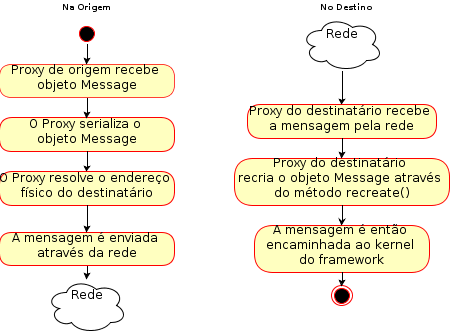
\includegraphics{fluxo_troca_msg.png}}
  \caption{Diagrama de fluxo de envio de mensagem entre dois \textit{environments} distintos.}
\label{fig:fluxo_troca_msg}
\end{figure}

\subsection{O método \emph{send} do \emph{Proxy}}

O método \textit{send} recebe como parâmetro um objeto do tipo \textit{Message} e o envia para o destinatário designado a ele. O próprio \textit{proxy} deve ser capaz de, em cooperação com o \textit{kernel} do \textit{framework}, resolver o endereço lógico do destinatário para seu correspondendte endereço físico, e realizar a comunicação.

O mesmoo método \textit{send} é utilizado para despachar componentes em uma migração. Mais detalhes sobre a implementação da migração de objetos é tratado na subseção~\ref{migrar_componentes}

\begin{figure}
  \centerline{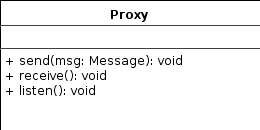
\includegraphics{uml_proxy_basico.png}}
  \caption{Diagrama de classes da classe \textit{proxy}.}
\label{fig:uml_proxy_basico}
\end{figure}

\subsection{O método \emph{receive} do \emph{Proxy}}

O método \textit{receive} do \textit{Proxy} do sistema é o método que é responsável por receber todas as mensagens externas direcionadas ao \textit{environment}. Este método deve executar ininterrupdamente durante todo o processo de simulação.

Para se evitar que o método \textit{receive} bloqueie a execução do sistema, este é executado de forma assíncrona aos demais componentes. Isto é feito utilizando a \textit{API} de manipulação de \textit{threads} de baixo nível da linguagem \textit{Python}.

O código listado no apêndice~\ref{appendix_proxy_example} ilustra uma versão bastante simplificada da implementação do método \textit{receive} de forma assíncrona usando a \textit{API} de baixo nível de \textit{threads} da linguagem \textit{Python}.

O construtor da classe (método \textbf{\_\_init\_\_}) recebe os parâmetros básicos para inicializar o \textit{proxy} e dispara uma chamada assíncrona (\textbf{thread.start\_new\_thread(...)}) passando como argumento uma referência para o método que se deseja executar de forma assíncrona (neste caso, o método \textbf{\_\_receiver\_\_}). Com o método \textbf{\_\_receiver\_\_} passa a ser executado ininterrupdamente, em paralelo à função que executou a instanciação do objeto \textit{Proxy}.

\section{Componentes \label{implement_components}}

Os componentes do \textit{framework} são descritos sobre o componente base \textit{Process}. Isto se dá porque o \textit{environment} deve ser capaz de lidar com qualquer tipo de componente de forma indistinta. Sendo assim, o \textit{environment} fica livre para manipular objetos de um mesmo tipo, cabendo a ele checar a especialização do tipo de cada objeto apenas no momento conveniente.

Novos componentes podem ser criados de duas maneiras: extendendo a classe base \textbf{\_\_Component\_\_} e criando um subtipo completamente novo, ou simplesmente encapsulando diversos componentes com determinadas características em um \textit{container} de componentes, deixando visível apenas seus parâmetros configuráveis e suas entradas e saídas.

\subsection{Migração de componentes \label{migrar_componentes}}

Todo objeto derivado da classe \textit{Component} deve contemplar a possibilidade de serialização de seu conteúdo. Isso se faz necessário porque é baseado na serialização de um componente que a sua migração é implementada.

Uma vez que o sistema identifica que um objeto deve migrar de seu \textit{environment} atual para um novo ambiente, uma série de ações são tomadas:

\begin{itemize}
	\item O componente em questão é marcado como \"em trânsito\".
	\item O objeto é serializado.
	\item Seus dados serializados são enviados, através do \textit{proxy} do \textit{environment} para o novo ambiente de execução.
	\item Uma vez em seu novo ambiente, o componente é reconstruído.
	\item As tabelas de endereço dos \textit{proxies} do sistema são atualizadas.
	\item O estado do componente é marcado como \"ativo\".
\end{itemize}

A partir da construção do \textit{middleware} de comunicação, composto pelos \textit{proxies} dos ambientes, a implementação da migração foi bastante simplificada. Como as suas construções são totalmente independentes, caso haja a necessidade de se atulizar ou trocar o sistema de comunicação ou mesmo o sistema de serialização dos componentes, se as interfaces dos objetos forem matidas, a funcionalidade de migração permanece consistente.

\section{Implementando o \emph{Environment}}

\section{Exemplos de aplicação}

Esta seção tem como fim demonstrar a estrutura básica de um código utilizando o \textit{framework} implementado durante este projeto. O que é apresentado são exemplos simples que visam apenas ilustrar o funcionamento do \textit{framework} desenvolvido, assim como ilustrar o uso da biblioteca de componentes do \textit{framework}.

\subsection{Uma aplicação típica}

O código ilustrado pela listagem~\ref{example_use_01} apresenta uma aplicação mínima de simulação utilizando o \textit{framework} desenvolvido neste trabalho.

As linhas [01] e [02] importam as bibliotecas necessárias para utilizar o \textit{framework}. A biblioteca \textbf{Simulator} é a responsável por gerenciar a simulação. Ela se encarrega de orquestrar a comunicação entre os componentes.

A biblioteca \textbf{base\_components} possui os componentes básicos para a construção de uma simulação. É com esses componentes que o modelo a ser simulado deve ser construído.


As linhas [07] e [08] criam funções que são passadas para o componente que será criado. Essas funções determinam o comportamento do componente durante a simulação. 

As linhas [11] e [12] criam dois componentes: uma fila de eventos e uma fonte geradora de eventos. Para a construção do gerador é passado como parâmetros as funções criadas nas linhas [07] e [08]. A expressão \textit{creation\_tax\_expression} rege sobre a frequência que cada novo evento é criado pelo gerador de eventos, enquanto a expressão \textit{execution\_time\_expression} representa o valor de cada evento criado. Este valor do evento é o que determina o custo do seu processamento pelo componente processador.

Um outro parâmetro passado durante a criação do componente \textbf{Source} é o parâmetro \textit{output}. Este parâmetro determina a qual componente a saída do gerador estará ligada. No exemplo aqui discutido, a saída do gerador está ligada à fila declarada na linha [11].

Na linha número [16] é declarado o componente \textbf{Process}, e é passado como parâmetro para este uma lista de todos os componentes que possuem suas saídas atreladas à entrada do processador.

Por fim, entre as linhas [18] e [21] é criado o componente \textit{Simulator}, responsável por gerir a simulação. Paar isto é passado ao contrutor do simulador uma lista com todos os componentes que contemplam a simulação. Com posse de uma instância do objeto \textit{Simulator}, é requerida a sua execução chamando o método \textit{run(...)}  e passando como parâmetro o número de passos a serem simulados.

As linhas [22] e [24] obtêem dados referente a simulação (o tamanho da fila de eventos, ao final da simulação) e devolvem para o usuário através da saída padrão.

\lstinputlisting[language=Python,
                 label=example_use_01,
                 caption="Exemplo de uma aplicação utilizando o \textit{framework} desenvolvido"]{example_use_01.py}

\subsection{O sistema de registro de execução da simulação}

Em ambos os exemplos ilustrados até então, o resultado da simulação era dado pelo tamanho da fila de eventos, que era aferida diretamente e impressa na saída padrão. Porém, o sistema desenvolvido possui uma ferramenta que possibilita traçar todas as atividades do sistema, além de acompanhar o ciclo de vida de cada componente ou evento do sistema.

Para habilitar a ferramenta de \textit{log} do sistema basta, ao se criar um objeto do tipo \textit{Simulator}, habiliatra o modo \textit{verbose}, passando um parâmetro extra \textbf{verbose=True}, além de passar como parâmetro um objeto do tipo \textit{file\_like\_object}, representando o arquivo onde o \textit{log} será armazenado.

Um exemplo de como instaciar um objeto \textbf{Simulator} para gerar um log de saída:

\begin{lstlisting}
# Cria um arquivo chamado simulation.log em /tmp
output_file = open('/tmp/simulation.log', 'w')
# Instaciar um objeto do tipo Simulator
simul = Simulator(components=[q1,q2,s1,s2], 
	              verbose=True, 
	              output_file=output_file)
\end{lstlisting}

Durante todo o processo de simulação, todas as atividadas (como criação de evento, entrada de um evento na fila, prcessamento de um evento, etc.) são registradas no arquivo de \textit{log} do sistema. Com isso, após a simulação, pode-se utilizar uma aplicação dedicada a ler este arquivo e estudar o comportamento do modelo durante a simulação.

\subsection{Escalabilidade do framework}

Em todos os exemplos ilustrados não há mençào sobre o número de nós no sistema. Quando uma execução é realizada desta maneira, o \textit{framework} assume que não existem mais nós no sistema, e a simulação se dá em apenas uma máquina.

Para se incluir mais nós no sistema de simulação, um parâmetro deve ser passado ao se instanciar o \texint{Simulator}. Este parâmetro, denominado \textit{cfg} contém as configurações do sistema físico, contando com descrições de todos os nós do sistema, tal como seus endereçoes físicos na rede. 

Este arquivo de configuração pode ser descrito tanto no formato \textit{xml} como no formato \textit{json}. Um exemplo de arquivo de configuração de um sistema distribuído é apresentado na listagem~\ref{nodes_cfg}.

\lstinputlisting[language=json,
                 label=nodes_cfg,
                 caption="Exemplo de arquivo de configuração dos nós da rede."]{distributed_01.json}

Uma vez que se deseja distribuir a simulação por entre os nós de um sistema distribuído basta, em posse do arquivo de mapeamento do sistema, passar o caminho para este arquivo como parâmetro \textit{cfg} na construção do objeto \textit{Simulator}.

Vale ressaltar que, da maneira que este \textir{framework} foi desenvolvido, para adicionar um nó extra ao sistema basta mapear o novo nó no arquivo de configuração do sistema, e o \textit{framework} fará a partição dos processos entre os nós automaticamente. Porém, um novo nó só pode ser adicionado ao arquivo de configuração antes do início da simulação. A atual concepção do sistema não permite a inclusão de nós durante o processo de simulação.

Todo nó do sistema que se disponibiliza a receber objetos para a simulação deve estar executando uma instância especial do \textit{framework}, responsável por receber os objetos despachados à ele e gerenciar a simulação.